\documentclass[11pt,fleqn]{book} % Default font size and left-justified equations

%%%%%%%%%%%%%%%%%%%%%%%%%%%%%%%%%%%%%%%%%%%%
%               Structure
%%%%%%%%%%%%%%%%%%%%%%%%%%%%%%%%%%%%%%%%%%%%
\input{sources/preamble.tex}

\begin{document}
	
	%\frontmatter
	%\begingroup
%\thispagestyle{empty}
%\begin{tikzpicture}[remember picture,overlay]
%  \coordinate [below=12cm] (midpoint) at (current page.north);
%  \node at (current page.north west)
%  {\begin{tikzpicture}[remember picture,overlay]
%      \node[anchor=north west,inner sep=0pt] at (0,0) {\includegraphics[width=\paperwidth]{images/background}}; % Background image
%\textsl{}
%      \draw[anchor=north] (midpoint) node [fill=ocre!30!white,fill opacity=0.6,text opacity=1,inner sep=1cm]{\Huge\centering\bfseries\sffamily\parbox[c][][t]{\paperwidth}{\centering Coding Interview Essentials\\[15pt] % Book title
%      {\Large - }\\[20pt] % Subtitle
%      {\huge Davide Spataro}}}; % Author name
%    \end{tikzpicture}};
%\end{tikzpicture}
%\vfill
%\endgroup


\includepdf[pages={2},fitpaper=true]{images/book_covers1.pdf}


	%\usechapterimagefalse % If you don't want to include a chapter image, use this to toggle images off - it can be enabled later with \usechapterimagetrue

	\chapterimage{images/header} % Table of contents heading image
	
	\pagestyle{empty} % No headers
	
	\tableofcontents % Print the table of contents itself
	
	%\cleardoublepage % Forces the first chapter to start on an odd page so it's on the right
	
	\pagestyle{fancy} % Print headers again
	

	%!TEX root = ../main.tex
%%%%%%%%%%%%%%%%%%%%%%%%%%%%%%%%%%
% Links:
%
% Difficulty: Easy/Medium
% Companies: 
%%%%%%%%%%%%%%%%%%%%%%%%%%%%%%%%%%

\chapterimage{header}

\chapter{Power set generation}
\label{ch:power_set}
\section*{Introduction}


\section{Problem statement}
Write a function that given a collection $S$ returns its power-set. A power-set of a collection $S$ is the set of all its ordered subsets including the empty subset and S itself. Subsets can appear in any order.

\begin{example}
	\hfill \\
	For the collection of characters $S=\{a,b,c\}$  both $P$ and $P'$ are two valid outputs of the function:
	\begin{equation*}
		P = \{\{\}, \{b,c\}, \{a\}, \{a,b\}, \{a,b,c\}, \{b\}, \{a,c\}, \{c\} \}
	\end{equation*}
	\begin{equation*}
		P' = \{\{\}, \{a\}, \{b\}, \{c\}, \{a,b\}, \{b,c\}, \{a,c\}, \{a,b,c\} \}
	\end{equation*}
	
\end{example}

\section{Clarification Questions}

\begin{QandA}
	\item What is the maximum size of the input?
	\begin{answered}
		\textit{The maximum number of element is strictly less than $n < 32$.}
	\end{answered}
	
	\item Are all the element in the collection distinct?
	\begin{answered}
		\textit{No, the elements are not necessarily distinct. $S$ can contain duplicates.
}
	\end{answered}
\end{QandA}

\section{Discussion}
There is one key point that should immediately be noticed:
\begin{itemize}
	\item \textbf{The powerset of a collection of $n$ elements has size $2^n$}. This fact should be immediately pointed out during the interview, stressing the fact that the constraint $n < 32$ is a strong hint towards the fact that an exponential solution is expected. Doing so shows knowledge on powersets and the ability to link and use that knowledge with the problem statement.
\end{itemize}

\subsection{Backtracking}
The solution to this problem is based on the fact that that during the generation of one of the elements of the power-set a decision has to be taken, for each element of the original collection, on whether to include or not into the subset.
We thus have two choices for each element of the input and that can be easily visualized drawing a tree as shown in Figure \ref{ref:power_set_decision_trees}.

One general way to deal with such type of problems is by using backtracking to try all possible decision paths for each of the elements. The proposed solution will incrementally construct one subset at the time, using an integer variable to keep track of which element we are currently deciding to include or exclude.
The base case of the recursion happen when there is no more decision to take, meaning that the current subset is ready to be included in the solution (it has been produced after $n$ decision steps).
The C++ code implementing the idea above is shown in Listing \ref{list:power_set_backtracking}.
\lstinputlisting[language=c++, caption="C++ to the power set generation using backtracking",label=list:power_set_backtracking]{sources/power_set/power_set_backtracking.cpp}

\begin{figure}
	\label{ref:power_set_decision_trees}
	\centering
	\includegraphics[scale=2.0]{sources/power_set/images/subsetTree}
	\caption{Decision tree for the power-set generation using backtracking.}
\end{figure}

The complexity of the backtrack solution is exponential i.e. $O(2^n)$ which is as good as it gets.

\subsection{Bit Manipulation}
Another approach that can be used to solve this problem is based on the fact that the values of the bits of the numbers $\{0,1,2,\ldots, s^n-1\}$  already provide all the information necessary to make decision weather to include or not an element from the input. In other words the set of numbers $P=\{0,1,2,\ldots, s^n-1\}$ is a powerset of $n$ bits. The binary representation of the numbers can be used to build one subset. For instance
given the input $S={a,b,c}$ the Table \ref{tab:mapping_value_bits} shows how numbers maps to their bit representation on how that can be used to construct one subset of the power-set of $S$. A $1$ means the corresponding element is taken, while a $0$ means it is excluded.

\begin{table}[H]
	\centering
	\begin{tabular}{|l|l|l|}
		\hline
		Value & Bits & Subset\\ \hline
		0     & 000  & $\{\}$\\ \hline
		1     & 001  & $\{c\}$\\ \hline
		2     & 010  & $\{b\}$\\ \hline
		3     & 011  & $\{b,c\}$\\ \hline
		4     & 100  & $\{a\}$\\ \hline
		5     & 101  & $\{a,c\}$\\ \hline
		6     & 110  & $\{a,b\}$\\ \hline
		7     & 111  & $\{a,b,c\}$\\ \hline
	\end{tabular}
	\label{tab:mapping_value_bits}
\end{table}

This idea can be used to write an algorithm in which all the numbers in the range $\{0,1,2,\ldots, s^n-1\}$ are considered and each of them maps to a subset of the final solution. 
The following code implements the idea above\footnote{Notice the usage of the \texttt{reserve} function that should be used in all those scenario when we already know the final size of the collection we are building. This saves times because avoids intermediate allocation and copy that must happen during the resize of the vector.}.

\begin{minipage}{\linewidth}
	\lstinputlisting[language=c++, caption="C++ to the power set generation using backtracking",label=list:power_set_backtracking]{sources/power_set/power_set_bit_manipulation.cpp}
\end{minipage}

\section{Common variations}

\section{Conclusion}

	%!TEX root = ../main.tex
%%%%%%%%%%%%%%%%%%%%%%%%%%%%%%%%%%
% Links:
%
% Difficulty: Easy/Medium Companies: 
%%%%%%%%%%%%%%%%%%%%%%%%%%%%%%%%%%

\chapterimage{header}

\chapter{Square root of an integer}
\label{ch:square_root}
\section*{Introduction}
The concept of square has root that go back to almost at the beginning of mathematics and it is not only one of the central operations in mathematics that
we use almost as often as addition or multiplication and division, but also at the core of countless of everyday gadgets and technology we use everyday like the radio and GPS systems, for instance.

The square root of a number $x$, denoted with the $\sqrt{}$ symbol, is formally defined to be a number $y$ such that $y^2 = x$.
For example the $\sqrt{4} = 2$ and $\sqrt{1253} \approx 35.3977$.

The problem in this chapter will make us derive an solution for the calculation of the square root of an integer.
Like almost every conding interview problems there are multiple possible solutions and approached we can take to tackle this problem. 
In Section \ref{} we discuss a simple and inefficient solution that works in $O(\sqrt(n))$
and then in Section \ref{} we will improve the runtime dramatically by deriving an elegant logarithmic time solution.

\section{Problem statement}
	\begin{exercise}
	Write a function that calculates the integral part of the square root of an integer.
	You cannot use any library functions.
	
	\begin{example}
		\hfill \\
		\begin{itemize}
			\item[-] 	\lstinline[columns=fixed]{my_sqrt(9)=3}: $\Longleftarrow $ $\ceil{\sqrt{9}}=3$
			\item[-] 	\lstinline[columns=fixed]{my_sqrt(11)=3}: $\Longleftarrow $
			$\ceil{\sqrt{11}}\approx\ceil{3.316624}=3$
			\item[-] 	\lstinline[columns=fixed]{my_sqrt(18)=4}: $\Longleftarrow $
			$\ceil{\sqrt{11}}\approx\ceil{4.242640}=4$
		\end{itemize}

	\end{example}
\end{exercise}
\section{Clarification Questions}
\begin{QandA}
	\item What is the maximum value the parameter $n$ can take?
	\begin{answered}
		\textit{The greatest input is guaranteed to be smaller than $2^{32}$.}
	\end{answered}
	
	\item Is $n$ guaranteed to be always positive?
	\begin{answered}
		\textit{Yes, there is no need to check for invalid input.}
	\end{answered}
\end{QandA}

\section{Discussion}
A brute-force solution is quickly derivable from the defintion of square root given above and the interviewer
is very likely expecting to see a it mentioned or appearing on the whiteboard
within the first 5 minutes of the interview. 

\subsection{Brute-Force}
We know from the definition given above that if $y$ is the square root of $x$ then $y^2 = x$. Moreover,
$y$ is an integer only when $x$ is a perfect square\footnote{$x$ is a perfect square if exists an integer $y$ such that $y^2=x$.}. 
If $x$ is not a perfect square than $y$ is real number and the following holds true
$\floor{y}^2 \leq x$ and $\ceil{y}^2 > x$. For instance the $\sqrt{5} \approx 2.2360$ and $2^2=4 \leq 5$ and $3^2=9 > 5$.
We can use this last property in a brute-force solution where we blindly loop all the integers $k=0,1,2,\ldots$ until 
the following property is true $k^2\leq n$ and $(k+1)(k+1) > n$.
A solution is guaranteed to be found because eventually $k$ will be equal to $\floor{y}$.
It should be immediately clear that no more than $\sqrt{n}$ numbers will be tested, therefore the time complexity of this approach is $O(\sqrt{n})$.

Listing \ref{list:square_root_brute_force} shows a C++ implementation of this idea.
Pay attention to the fact that the variable $i$ has a type that is larger in size w.r.t. an
$int$. This is necessary in order to prevent overflows during the calculation of $i^2$. 
One of the constraint of the problem is that the largest input can be $n=2^{32}-1$; if we square that number the result does not fit in a $4$ bytes int.


	\lstinputlisting[language=c++, caption=$O(\sqrt{n})$ solution to the problem of finding the square root of an integer.,label=list:square_root_brute_force]{sources/square_root/square_root_brute_force.cpp}


\subsection{Logarithmic Solution}
Binary search can be effectively used to solve this problem and tn order to show that, we are going
to look at the problem from a slightly different angle. Let 
\begin{equation}
	F(k)=\begin{cases} 
	0 & k^2 \leq n \\
	1 & k^2 > n
\end{cases}
\label{eq:square_root_piecewice}
\end{equation} 
be a piece-wise function that partition the search space $[0\ldots n]$ into two parts (See Table
\ref{tab:sqrt_split_space}):
	\begin{itemize}
      \item [-] the numbers  less or equal than $\sqrt{n}$
      \item [-] the numbers strictly greater or equal than $\sqrt{n}$
	\end{itemize}
The answer to this problem is the greatest value $k$ s.t. $F(k) = 0$. 
Note that every number in the left part of the search space, $0 \leq l \leq \floor{n}$ has $F(l) = 0$, while the elements in the right side,$\floor{n}+1 \leq r \leq n$, have $F(r) = 1$.
Because the function $F(k)$ splits the search space into two parts, we can use
binary search to find the end of the first partition. 
We can do that because if we pick an integer from in $[0,n]$, say $k$, and $F(k) = 1$ we know that $k$ is not the solution and crucially also that
all the values greater than $k$ are not good candidates because they all belong to the right partition.
On the other hand if $F(k) = 0$, we know that either $k$ is the solution but also that all the elements smaller than $k$ are not good candidates either.
The idea above is implemented in Listing \ref{list:square_root_binary_search}. 
The algorithm works by iteratively searching in a
incrementally smaller subinterval defined by the variables $l$ and $r$. 
At each iteration we test the middle element of $[l,r]$ (the variable \inline{middle}), and this can lead to one of the following three scenarios:
\begin{enumerate}
 	\item $(middle)^2  = n \longrightarrow$: $middle$ is the solution. $n$ is a perfect square and
 	$\sqrt(n)=middle$
 	\item $(middle)^2  > n \longrightarrow$: $middle$ is not the solution and we can also exclude
 	all numbers $k \geq middle$ from the search (by doing $r = middle-1$).
 	\item $(middle)^2  < n \longrightarrow$: $middle$ is the best guess we have found so far (it might be the solution). We can
 	however, exclude all numbers smaller than $middle$, $k < middle$, from the next iterations (by doing $l = middle+1$).
\end{enumerate}
Pay attention to the way the midpoint between $l$ and $r$ is calculated. 
It is common to see it calculated by using the following formula:$(l+r)/2$. This however can leade to overflow problems when $l+r$ does not fit in a \inline{int}.
The complexity of this approach is logaritmic in $n$. A good improvement w.r.t. to the complexity of the brute-force solution.

\begin{table}
	\centering
	\begin{tabular}{|c|c|c|c|c|c|c|}
		\hline
		$0$ & $1$ & $2$   & $\floor{\sqrt{n}}$ & $\floor{\sqrt{n}}+1$ & \ldots   & $n$ \\ \hline
		$0$ & $0$ & \ldots & $1$ & $1$ & \ldots & $1$   \\ \hline
	\end{tabular}
	\caption{Partition of the search space according to the function in Eq.
	\ref{eq:square_root_piecewice}}
	\label{tab:sqrt_split_space}
\end{table}


	\lstinputlisting[language=c++, caption=$O(log_2(n))$ solution to the problem of finding the square root of an integer.,label=list:square_root_binary_search]{sources/square_root/square_root_binary_search.cpp}



\section{Conclusion}

	%!TEX root = ../main.tex
%%%%%%%%%%%%%%%%%%%%%%%%%%%%%%%%%%
% Links:
%
% Difficulty: Easy/Medium Companies: 
%%%%%%%%%%%%%%%%%%%%%%%%%%%%%%%%%%

\chapterimage{header}

\chapter{Two string anagram}
\label{ch:two_string_anagram}
\section*{Introduction}
Given a certain a certain word, you can construct other words by only changing the arrangements of its characters.
For instance from the characters in \textit{alerting} you can spell the following words:
\begin{enumerate*}
	\item \textit{altering}
	\item \textit{integral}
	\item \textit{relating}
	\item \textit{triangle}
\end{enumerate*}.
Words sharing the same characters-set are called anagrams. 

Being able to create good anagrams,
especially ones reflecting or commenting the word they are generated from (for instance turning
\textit{Madam Curie} into \textit{Radium came}) is regarded as difficult task.
Computers have been used for long time to find anagrams in long texts as well as to generate the so
called anagram dictionaries \footnote{special kind of dictionary where all the letters in a word and
all their transposition are arranged in alphabetical order} that are often used in games like
Scrabble. Often, at the core of such application lies an efficient algorithm for determining if a word is an anagram.

The problem discussed in this chapter is about anagrams, and more specifically about determining how many 
modification you need to make to a word in order to make it the anagram of a
another given word. It is regarded as an easy problem mostly because the statement is straightforward to
understand, the concept of anagram is part of the common knowledge and no particular insights or particularly
tricky reasoning is required in order to obtain an efficient solution. 
However, it has been frequently asked in coding interview, especially during the preliminary stages.
Moreover, despite its simplicity, there is more than one neat and elegant approach leading to an efficient
solution to this problem.
In the rest of the chapter we are going to have a look at three
solutions, from the slow and easy to understand brute-force in Section \ref{sec:anagrams:bruteforce} to a faster using
sorting in Section \ref{sec:anagrams:sorting}, and finally, to the optimal solution running in linear time in Section
\ref{sec:anagrams:histograms}. 

\section{Problem statement}
	\begin{exercise}
	Write a function that given two string, $a$ and $b$ of length $n$ and $m$, respectively, determines the minimum
	number of character substitution, $C(s, i, c)$, necessary to make the string $a$ an anagram of the string $b$.
	Two strings are said to be anagrams of one another if you can turn the first string into the second by
	rearranging its letters. A substitution operation $C(s,i,c)$ modifies the input string $s$, by changing its $i^{th}$ character
	into $c$. Notice that deletions or additions of character is not allowed. The only operation you can do is change a character of the first string into another one. 
	You can perform any number of modification.

	In other words, what is the minimum number of  characters of the input strings that need to be
	modified (no addition or deletion)  so that $a$ becomes an anagram of $b$?

	\begin{example}
		\hfill \\
		\begin{itemize}
			\item[] 	a = "aaa"
			\item[] 	b = "bbb"
		\end{itemize}
		The answer for this case is: 3. All the character of the first string needs to be changed to \textit{'b'}.
		\label{ex:anagrams:example1}
	\end{example}

	\begin{example}
		\hfill \\
		\begin{itemize}
			\item[] 	a = "tear"
			\item[] 	b = "fear"
		\end{itemize}
		The answer for this case is: 1. All it is necessary is turning the first letter of $a$ into an \textit{'f'}.
		
	\end{example}

	\begin{example}
		\hfill \\
		\begin{itemize}
			\item[] 	a = "Protectional"
			\item[] 	b = "Lactoprotein"
		\end{itemize}
		The answer for this case is $0$ because $a$ is already an angram of $b$.
	\end{example}
\end{exercise}

\section{Clarification Questions}

\begin{QandA}
	\item Are the letters of the string always only letters from the English alphabeth? 
	\begin{answered}
		\textit{Yes, letters are always from the english alphabet.}
	\end{answered}
	
	\item Should the function be case sensitive? 
	\begin{answered}
		\textit{No, in particular the letters are always lower case.}
	\end{answered}
	\item Can the input string be modified? No, the input is immutable.
	\begin{answered}
		\textit{No, the input strings are immutable.}
	\end{answered}

	\item What value should be returned when there is no solution?
	\begin{answered}
		\textit{In such case you can return $-1$.}
	\end{answered}
\end{QandA}

\section{Discussion}
Let's start by first quickly review what the word anagram means in this case. For $a$ to be an anagram
of $b$, it has to be the case that exists an arrangement of characters in $a$ that is equal to $b$.
In other words, the question to which we need to answer is: is it possible to shuffle the character of $a$ such that we obtain $b$?
For this to be case, it must be that $a$ and $b$ contains the same set of characters meaning that sorting both $a$ and $b$
lead to two the same strings. 
Moreover as a consequence of the fact that no addition or deletion
is allowed, $a$ and $b$ must have the same length. 
But if they have the same length then it is always
possible to solve this problem because in the worst case, we can modify every letter in $a$ (see Example \ref{ex:anagrams:example1}).
Thus, the only case when the problem has no solution has been isolated i.e. if the input string differes in length we must return $-1$ otherwise we can proceed with our calculation knowing that a solution exists.


\subsection{Brute-Force}
\label{sec:anagrams:bruteforce}
Probably one of the first options coming to mind is the brute force solution where we generate all possible arrangements of the letters in $a$, and
for each arrangement we calculate the number of modifications necessary for converting it into $b$. The key idea is that the cost of transforming a string into
another equals to the numbers positions having different letters. For instance the cost of transforming "abcb"
into "bbbb" is $2$ because the two strings differ in the first and third letter. 

Despite its conceptual simplicity this approach is to be considered poor because the number
of arrangements to be checked grows very fast with the length of the input string (as fast as $n!$).
Moreover, its implementation  is not straightforward because the generation of all permutation is not easy do to
by hand unless you use a third party library capable of doing that or certain languages like C++ that offers standard library functions devoted to this purpose (\lstinline[columns=fixed]{std::next_permutation(...)}\footnote{\url{https://en.cppreference.com/w/cpp/algorithm/next_permutation}}).

Listings \ref{list:two_string_anagram_bruteforce} shows a C++ implementation of the idea above using \lstinline[columns=fixed]{std::next_permutation}.
\lstinputlisting[language=c++, caption="Brute force C++ solution to the two string anagram problem.",label=list:two_string_anagram_bruteforce]{sources/two_string_anagram/two_string_anagram_brute_force.cpp}


\subsection{Sorting}
\label{sec:anagrams:sorting}
The brute-force solution does a lot of superfluous work because it tries to find a permutation of the string $a$
requiring  minimal modifications to be morphed into b.
But, is really necessary to try to turn $a$ into exactly $b$, or is it sufficient to turn $a$ into a particular permutation of $b$? 
Afterall being an anagram is a transitive property meaning that if $a$ is a permutation of $b$ and $b$ is a prtmutation of $c$ then $a$ is also a permutaion of $c$. 
By definition an anagram of $b$ is any permutation of its characters, meaning that also the permutation in which the characters of $b$ are sorted is a valid
anagram. It is much easier if we try to modify $a$ into this sorted version of $b$ rather than to exactly $b$ because all we need to do it to create
a copy of $a$ and $b$, sort both of them and then calculate the letter by letter difference.
This approach works because if $x$ is an anagram of $b$ then $x$ is also an
anagram of \inline{sort(b)}. In other words, it does not matter how the characters are arranged in $a$ and $b$, the only thing that matters is the set of characters
appearing in $a$ and $b$. Listings \ref{list:two_string_anagram_sorting} shows a C++ implemenetation of the idea above. 
Note that if the input was mutable, then the additional space occupied by the copies of the string
could have been avoided. The complexity of the idea above is $O(n log(n))$(because of sorting) time and $O(n)$ space (because of the copies of the input).

\begin{minipage}{\linewidth}
 	\lstinputlisting[language=c++, caption="Brute force C++ solution to the two string anagram problem.",label=list:two_string_anagram_sorting]{sources/two_string_anagram/two_string_anagram_sorting.cpp}
\end{minipage}

\subsection{Histograms}
\label{sec:anagrams:histograms}
There is another bit of information that is not yet used i.e. the fact that the set from which the
letters (the alphabet) are taken from is really small. 
If the only thing that matters is the set of characters appearing in $a$ and $b$,
then we can use the same idea used at the core of bucket sort\footnote{\url{https://en.wikipedia.org/wiki/Bucket_sort}} to finally achieve a linear time solution.
To solve this problem efficiently it is then sufficient  to calculate the frequencies of the character in $a$, $F_a$, and $b$, $F_b$.
If $F_a$ and $F_b$ are the same, then $a$ is an anagram of $b$ otherwise then it must be that either some character is appears a different number of times in both strings.
All it is needed is modifying $a$ such that the frequencies of $F_a$ and $F_b$ match exactly. 
But how many operations are necessary to do so?  In order to get this answer it is useful to look at
the difference of the two frequencies arrays $D = F_a - F_b$:
\begin{equation*}
	 D = \{D[\mathrm{a}] = (F_a[\mathrm{a}] - F_b[\mathrm{a}]), D[\mathrm{b}] = (F_a[\mathrm{b}] - F_b[\mathrm{b}]), D[\mathrm{c}] = (F_a[\mathrm{c}] - F_b[\mathrm{c}]), \ldots, D[\mathrm{z}] = (F_a[\mathrm{z}] - F_b[\mathrm{z}])\}
\end{equation*}
First of all notice that $\sum_{\mathrm{a}}^{\mathrm{z}} D = 0$. Moreover, if an element of $D$ is greater than zero, than this means that $a$
has an excess of the corrensponding letter, and on the contrary if it is less than zero, it means $a$
has a deficit of that letter.
What can be done is to turn the letters in excess into letters that
are missing and that is possible since $\sum_{\mathrm{a}}^{\mathrm{z}} D= 0$.
The answer to this problem is the sum over the positive (alternatively negative) numbers of $D$. 
Listings \ref{list:two_string_anagram_histogram} shows a possible implemenetation of the idea above.
Notice how the array of differences of frequencies $D$ can be easily calculated without explicitelly
computing the frequencies for $a$ and $b$ but by simply adding a frequency for a letter appearing in $a$
and subtracing it for letters in $b$. 
First of all notice that $\sum D = 0$. Moreover, if an element of $D$ is greater than zero, than this means that $a$
has an excess of the corrensponding letter, and on the contrary if it is less than zero, it means $a$
has a deficit of that letter.
What can be done is to turn the letters in excess into letters that
are missing and that is possible since $\sum D = 0$.
The answer to this problem is the sum over the positive (alternatively negative) numbers of $D$. 
Listings \ref{list:two_string_anagram_histogram} shows a possible implemenetation of the idea above.
Notice how the array of differences of frequencies $D$ can be easily calculated without explicitelly
computing the frequencies for $a$ and $b$ but by simply adding a frequency for a letter appearing in $a$
and subtracing it for letters in $b$. 
The complexity of this approach is $O(n)$ in time and $O(1)$ in space. We cannot do better than this because all characters in the input strings must be at least accessed once in the worst case.

\begin{minipage}{\linewidth}
	\lstinputlisting[language=c++, caption="C++ solution to the two string anagram problem using the histogram approach.",label=list:two_string_anagram_histogram]{sources/two_string_anagram/two_string_anagram_histogram.cpp}
\end{minipage}

\section{Conclusion}
	%!TEX root = ../main.tex
%%%%%%%%%%%%%%%%%%%%%%%%%%%%%%%%%%
% Links: https://www.geeksforgeeks.org/count-pairs-with-given-sum/
% https://algorithms.tutorialhorizon.com/given-an-array-and-a-number-k-check-for-pair-in-array-with-sum-as-k-in-onlgn/
% https://coderbyte.com/algorithm/two-sum-problem https://en.wikipedia.org/wiki/Subset_sum_problem
%
% Difficulty: Easy Companies: Microsoft, Amazon, Google
%%%%%%%%%%%%%%%%%%%%%%%%%%%%%%%%%%

\chapterimage{header} % Table of contents heading image

\chapter{Two numbers sum problem}
\label{ch:two_numbers_sum}
\section*{Introduction}
This chapter addresses one of the most frequently posed problems during the early stages of the coding interview process: two numbers sums.  The problem is hard enough to require non-trivial insights in order to be able to write a non-trivial solution but, at the same time, it is not so hard that it would take a candidate hours to come up with something meaningful to say or to write. It's ubiquity also means that any interviewer will expect a candidate to be at least familiar with the issues and able to present multiple paths to solution. 

We are going to look at several possible solutions.

First, the inefficient brute force approach which we will subsequently refine it into a fast and time-optimal one).
Then,  a radically different approach based on sorting which [AGAIN SOMETHING ABOUT WHY THIS?].
Finally, condensing the strengths of all the previous solutions into a time and space optimal solution that will likely perform best in an interview context. As we will see, this final solution is efficient and not terribly difficult to write and explain; key elements for success in any coding interview.


\section{Problem statement}

\begin{exercise}
	Write a function that takes an array of integers $A$ of size $n$ and an integer $T$, and returns \textbf{true} if the sum of any two distinct elements $I$ is equal to $T$, \textbf{false} otherwise.

	More formally: Given an array $=\{a_1,...,a_n\}$ and $T$, where $a_i, T \in
	\mathcal{N}$, return:
	\begin{itemize}
		\item  \textbf{true} if $\: \exists \;i,j \:\: i \neq j$ s.t. $a_i+a_j = T$
		\item  \textbf{false} otherwise
	\end{itemize}
	

	\begin{example}
	\hfill \\
		Given $A=\{9, 4, 17, 42, 36, -3 ,15\}$ and $T=14$, the function returns \textbf{true} because we can obtain $14$ by summing
		up together the elements $17$ and $-3$.
		If $T=17$ the answer is \textbf{false}.
	\end{example}

	\begin{example}
	\hfill \\
		Given $A=\{1,3,7\}$ and $T=8$, the function returns \textbf{true} because we can obtain $8$ by summing
		up together the elements $7$ and $1$. If $T=6$ the answer is \textbf{false}.
	\end{example}

\end{exercise}	


\section{Clarification Questions}
\begin{QandA}
	\item \begin{questionitem} \begin{question} Is the input array modifiable?  \end{question} 	 
    \begin{answered}
		\textit{Yes, the input array can be modified.}
	\end{answered} \end{questionitem}	
	\item \begin{questionitem} \begin{question} Are the integers guaranteed to be all positive or all negative?   \end{question} 	 
    \begin{answered}
		\textit{No, $A$ can contain positive or negative numbers.}
	\end{answered} \end{questionitem}
	\item \begin{questionitem} \begin{question} Are the values in $A$ guaranteed to be from a given range?  \end{question} 	 
    \begin{answered}
		\textit{No, the input is arbitrary. No assumption can be made on the magnitude of the elements of $A$.}
	\end{answered} \end{questionitem}
	\item \begin{questionitem} \begin{question} Can a pair be made from an element and itself?  \end{question} 	 
    \begin{answered}
		\textit{No, the pair's elements should be distinct. You cannot use the same element $a_i$ twice. You can however use two elements at indices $i$ and $j$ s.t. $i \neq j$ and $a_i=a_j$.}
	\end{answered} \end{questionitem}
	\item \begin{questionitem} \begin{question} Are all elements in the array unique?  \end{question} 	 
    \begin{answered}
		\textit{No, duplicates are allowed.}
	\end{answered} \end{questionitem}
	\item \begin{questionitem} \begin{question} Is the input sorted?  \end{question} 	 
    \begin{answered}
		\textit{No, the ordering of $A$ is arbitrary.}
	\end{answered} \end{questionitem}
	\item \begin{questionitem} \begin{question} Shall the function integer overflow be considered when performing the sum of two integers? Is it possible for two elements of $A$ to sum up to a value that does not fit in a standard \inline{int}?  \end{question} 	 
    \begin{answered}
		\textit{No, you do not need to worry about overflow.}
	\end{answered} \end{questionitem}
\end{QandA}


\section{Discussion}

%%%%%%%%%%%%%%%%%%%%%%%%%%%%%%%%%%%%%%%
%        quadratic solution
%%%%%%%%%%%%%%%%%%%%%%%%%%%%%%%%%%%%%%
\subsection{Brute-force}
\label{sec:two_numbers:bruteforce}

The brute force solution is straightforward because it consists of a direct application of the formal problem statement. 
The solution space consists of all possible ordered pairs $(a_i,a_j)$, $i < j$. 
Two nested loops can be used to enumerate all those pairs, and, for each of them, we can check whether their sum is equal to $T$: if that is the case,
then   \textbf{true} can be immediately returned, otherwise, if we have checked every possible pair and none of them was good, then we can return  \textbf{false}.
You will find an a fomalization and an implementation of this idea in Algorithm \ref{algo:two_number_sum_bruteforce}
and Listing \ref{list:two_number_sum_bruteforce}), respectively.

\begin{algorithm}
	\SetAlgoLined \SetKwFunction{FMain}{solveQuadratic}
	
	\KwIn{$ A $ \tcp{An array $A$ of length $n$}} \KwIn{$ T $ \tcp{An integer $T$}}

	\Fn{\FMain{$A,T$}}{
	
		%\Output{true if two distinct element of $A$ sum to $T$}
		
		\For{$i\leftarrow 0$ \KwTo $n-1$} {\For{$j\leftarrow i+1$ \KwTo $n$} {\If{$a_i + a_j =
		T$}{\Return True \;}}} \Return False \;}\textbf{End Function}
	
		\caption{Two loops, quadratic solution to the question in Section \ref{ch:two_numbers_sum} }
		\label{algo:two_number_sum_bruteforce}
\end{algorithm}


\lstinputlisting[language=c++, caption="C++ solution of the two number sum problem with a brute force approach.",label=list:two_number_sum_bruteforce]{sources/two_numbers_sum/brute_force.cpp}

The time complexity of this solution is $O(n^2)$ because there is a quadratic number of
ordered pairs and in the worst case, we will look at \textbf{all} of them.

The number of iterations of the internal loop depends on the value of $i$ and
it is described by the function: $f(i) = n-i-1$. The total number of iterations the second
loop runs in the worst case is the the sum of $f(i)$ for all values of $i$: 
$\sum_{i=0}^{n-2} f(i) = (n-1) + (n-2) + (n-3) \ldots + 1 =\sum_{x=1}^{n-1} x= \frac{n(n-1)}{2} = O(n^2)$

The space complexity is $O(1)$.



\subsection{Hashing}
\label{sec:two_numbers:hashing}
The internal loop of the brute force solution above can be eliminated entirely with the help of a hash table.
The key insight is that if a solution exists involving $a_i$ then it must be the case that  exists another element $a_j  = a_i-T$ with $i > j$. 

What this means in practice is that we can loop through $A$ one element at a time and keep track in a lookup table of all the elements seen so far so that the lookup operation for the aforementioned element $a_j$ can be performed in constant time.

Algorithm \ref{algo:two_number_sum_hashset} and Listing \ref{list:two_number_sum_hashing} shows this idea in code.

%%%%%%%%%%%%%%%%%%%%%%%%%%%%%%%%%%%%%%%
% two_numbers_sum_hashset       
%%%%%%%%%%%%%%%%%%%%%%%%%%%%%%%%%%%%%%
\begin{algorithm}
	%	\KwData{} \KwResult{Tr }
	\KwIn{$ A $ \tcp{An array $A$ of length $n$}} \KwIn{$ T $ \tcp{An integer $T$}} \KwOut{true if
	two distinct element of $A$ sum to $T$, False otherwise} \SetKwFunction{FMain}{solveHashSet}
	
    \Fn{\FMain{$A,T$}}{H $\longleftarrow$ \CreateHashSet \;
	
		\For{$i\leftarrow 0$ \KwTo $n$} {target $\leftarrow$ $(T-a_i)$ \eIf{H.find(target)} {\Return
		True} {H.insert($a_i$)}} \Return False\;}\textbf{End Function}

		\caption{Hashset, linear solution to the \textit{two number sum} question in Section
		\ref{ch:two_numbers_sum}.}
		\label{algo:two_number_sum_hashset}
\end{algorithm}


\lstinputlisting[language=c++, caption="C++ solution of the two number sum problem using hashing.",label=list:two_number_sum_hashing]{sources/two_numbers_sum/hashset.cpp}

The time complexity of this approach is $O(n)$ (technically it is linear on average due to the complexity of lookups in hash tables) because the input array is scanned once and for each
of its elements, only one lookup and insertion are performed in the hash table (both operations costing constant time on average).

The space complexity
is also $O(n)$ as, in the worst case scenario,  the whole input array is stored in the lookup table.

A common mistake when solving this problem using this approach is to insert the whole input array into the lookup table, and only after searching for $(T-a_i)$.
The mistake becomes evident when $T$ is an even number ($2 | T$) and $\frac{T}{2}$ appears in $A$  exactly once, at index $k$ i.e. $a_k = \frac{T}{2}$ causing \inline{H.find(T-a_k)} to return \textbf{true}, which is wrong because this corresponds to a solution where we sum $a_k$ twice to obtain $T$.

For instance, when $A=\{1,2,5,4\}$ and $T=10$ this approach wrongly returns \textbf{true}, even if there are not two elements at distinct indices in $A$ whose sum is $T$ (we would use $5$ twice to obtain $10$).
\begin{example}
	\hfill \\ 
	\begin{itemize}
		\item[] $A=\{1,2,5,4\}$
	\item[] $T = 10$
\end{itemize}
	Algorithm \ref{algo:two_numbers_sum_hashset_wrong} wrongly return true even if there are not two
	distinct elements whose sum is $10$.
\end{example}


%%%%%%%%%%%%%%%%%%%%%%%%%%%%%%%%%%%%%%%
% two_numbers_sum_hashset_wrong       
%%%%%%%%%%%%%%%%%%%%%%%%%%%%%%%%%%%%%%
\begin{algorithm}
	\SetKwInOut{Input}{input} \SetKwInOut{Output}{output}
	\SetKwFunction{CreateHashSet}{CreateHashSet<int>} \Input{An array $A$ of length $n$} \Input{An
	integer $T$} \Output{true if two distinct element of $A$ sum to $T$}
	
	\SetKwFunction{FMain}{solveHashSet} \Fn{\FMain{$A,T$}}{H $\longleftarrow$ \CreateHashSet \;
		\tcp{Add the whole array in the hashset}
		\For{$i\leftarrow 0$ \KwTo $n$} {H.insert($a_i$)\;}
		
		\For{$i\leftarrow 0$ \KwTo $n$} {target $\leftarrow$ $T-a_i$ \; \If{H.find(target)} {\Return
		True}} \Return False\;}\textbf{End Function}
		\caption{Hashset, linear solution to the \textit{two number sum} question in Section
		\label{algo:two_numbers_sum_hashset_wrong}
	\ref{ch:two_numbers_sum} }
\end{algorithm}


\subsection{Sorting and binary search}
\label{sect:two_number_problem_binary_search}

As with countless other problems on arrays, sorting the input often leads to a faster and more efficient solution. 

We can start by asking ourselves how the problem changes if  $A$ is sorted. Sorted arrays are naturally associated with binary search as many problems can be solved efficiently by pairing sorting and binary search on arrays. 
This problem is no different therefore we can use binary search if $A$ is sorted to substitute the internal loop of the brute force solution presented [above](). This way, we lower the overall complexity  to $O(n log(n))$; it costs
$O(n log(n))$ to sort the input array in the first place, and the actual search consists of $n$ binary
searches, each of them costing $O(log(n))$. 

The space complexity is $O(1)$ because no additional space is required as the array is sorted in place.

Listing \ref{list:two_number_sum_sorting} shows a C++ implementation of this idea. Note that it uses \inline{std::binary_search} from the C++ standard library and that a possible follow-up question might be to show your own version of the binary search algorithm.



\lstinputlisting[language=c++, caption="C++ solution of the two number sum problem with sorting and binary search.",label=list:two_number_sum_sorting]{sources/two_numbers_sum/two_numbers_sum_sorting.cpp}


\subsection{Sorting and two pointers technique}
\label{sec:two_numbers:twopointers}

There is a variation to the to the approach described in Section
\ref{sect:two_number_problem_binary_search} which still involves sorting but uses a two-pointers
technique instead of binary search to finish the job. 

The key idea is that, once $A$ is sorted, the algorithm initializes
two pointers: one starting at the beginning ($p_s$) and the other at the end ($p_e$) of the array respectively.
It continues by looking at the sum of the two elements pointed by the two pointers and moving one of
the two at each step using the following logic: 
\begin{itemize}
	\item if $a[p_s]+a[p_e] = T$ a solution has been found. The algorithm returns true.
	\item if $a[p_s]+a[p_e] > T$, $p_e=p_e-1$. The right pointer is moved to the left. 
	Moving	$p_e$ to the left has the effect of making the sum of the values pointed by the two pointers smaller (this has an effect at the next iteration). 
	\item if $a[p_s]+a[p_e] < T$, $p_s=p_s+1$. The right end pointer is moved to the left. Moving $p_s$ to the right has the effect of making the sum of the values pointed by the two pointers larger. 
\end{itemize}



Listing \ref{list:two_number_sum_two_pointers} shows an implementation of the idea above. Note that compared to the solution using the binary search, this one is shorter and simpler to write. Moreover, it does not use library functions. 

\lstinputlisting[language=c++, caption="C++ solution of the two number sum problem with the two pointers tecnique.",label=list:two_number_sum_two_pointers]{sources/two_numbers_sum/two_numbers_sum_two_pointers.cpp}

Despite the fact that the overall time complexity is still $O(n log(n))$, this solution is likely to be faster than
using binary search due to the fact that the array is scanned linearly (which makes caches happier) by the two pointers and not in the scattered way of binary search.

%%%%%%%%%%%%%%%%%%%%%
\section{Common Variations}
\subsection{Four numbers sum problem}
\label{sec:four_number}

\subsection{Problem statement}

\begin{exercise}
Write a function that takes four arrays of integers, $A,B,C,D$ and a integer $T$,
and returns how many distinct tuple $(i,j,k,l)$ where exist such that $A_i+B_j+C_k+D_l = Y$.

\begin{example}
\hfill \\
Given:
	\begin{itemize}
		\item[-] 	$A=\{1,2\}$,
		\item[-] 	$B=\{-2,-1\}$,
		\item[-] 	$C=\{-1,2\}$,
		\item[-]	$D=\{0,2\}$, and 
		\item[-] 	$T = 0$
	\end{itemize}
The answer is $2$ because the only two valid tuples are:
\begin{enumerate}
	\item $(0,0,0,1)$: $A_0 + B_0 + C_0 + D_1 = 1 + (-2) + (-1) + 2 = T = 0$
	\item $(1,1,0,0)$: $A_1 + B_1 + C_0 + D_0 = 2 + (-1) + (-1) + (-1) = T = 0$
\end{enumerate}
\end{example}
\end{exercise}

\subsection{Na\"ive $O(n^4)$ solution}
We can solve this problem very easily by using the same approach we have described in Section \ref{sec:two_numbers:bruteforce}.
The idea is that we can use four nested loops and enumerate all possible 4-elements tuples of indices. Listing \ref{list:two_number_sum_naive} shows how this can be implemented.
This is not, however,  the fastest solution we can come up with as it has a time complexity of $O(n^4)$

\lstinputlisting[language=c++, caption="Brute force na\"ive solution to the four numbers sum problem.",label=list:two_number_sum_naive]{sources/two_numbers_sum/variations/four_number_sum/four_number_sum_solution1.cpp}

Needless to say, that this is not the fastest solution we can come up with, considering it has a time complexity of $O(n^4)$.

\subsection{$O(n^3)$ solution}
The trivial solution shown in Listing \ref{list:two_number_sum_naive} can be improved by using a similar approach to the one we used to improve the brute-force 
quadratic time solution for the two numbers problem in Listing \ref{list:two_number_sum_bruteforce} and to the linear time (and space) in Listing \ref{list:two_number_sum_hashing}.

The idea is that the inner-most loop is searching for a value $D_l = x$  s.t. if it summed to $A_i+B_j+C_k$ gives us $T$; in other words: $x+(A_i+B_j+C_k)=T$.
Therefore $x = T-(A_i+B_j+C_k)$. If there is a way of avoiding a linear search in the array $D$ for such a value, then we could bring down the complexity from $O(n^4)$ to $O(n^3)$.

This is possible if we use a hash map. If we create a hashmap mapping the value of $D$ and to their frequencies, the inner-most loop of the $O(n^4)$ solution above can be substituted with a query to the hashmap which runs in constant time (on average). 

Listing \ref{list:two_number_sum_cubic} shows an implementation of this idea. 
Note that, in order to obtain the maximum saving in terms of work avoided, the arrays are rearranged in such a way that $D$ is the longest of the four input arrays. 

\lstinputlisting[language=c++, caption="Brute force cubic time solution to the four numbers sum problem.",label=list:two_number_sum_cubic]{sources/two_numbers_sum/variations/four_number_sum/four_number_sum_solution2.cpp}


\subsection{$O(n^2)$ solution using hashing}

This problem can be however be solved  more efficiently in quadratic time if we use hashmaps by holding all  
the frequencies of all the values we can obtain by summing up any two elements of $A$ and $B$ and of $C$ and $D$.
The key idea is that we can build two distinct hashmaps:
\begin{itemize}
	\item $AB$: holding the frequencies of the values obtainable by summing any two elements of $A$ and $B$
	\item $CD$: holding the frequencies of the values obtainable by summing any two elements of $C$ and $D$.
\end{itemize}

The space required for both $AB$ and $CD$ is quadratic, which is more than the space used by any of the previous solutions, but this extra space
also enables us to solve this variation in quadratic time. 

The idea is that we are going to spend $O(n^2)$ time to construct both $AB$ and $CD$
and then again $O(n^2)$ to calculate the final answer 
by searching into $CD$ for the value $T-y$ where $y$ is an element of $AB$. 
If such a value exists in $CD$ it means that there exists one element in  $A$ and one in $B$ such that they sum up to $y$ and
one element $C$ and one in $D$ such that they sum up to $T-y$. Summing all these elements up gives: $y+T-y = T$.
This approach is shown in Listing \ref{list:two_number_sum_quadratic}. 

\lstinputlisting[language=c++, caption="Quadratic time solution to the four numbers sum problem.",label=list:two_number_sum_quadratic]{sources/two_numbers_sum/variations/four_number_sum/four_number_sum_solution3.cpp}

Note that the first thing we do is to fill $AB$ by looping over all possible pairs of elements from $A$ and $B$.
We then do the same thing for $CD$, and finally, in the last loop, we take care of calculating the answer by searching, for each element $(k,v)$ of $AB$, where $k$ is the sum obtained by one element of $A$ and one of $B$, and $v$ is the number of ways we can obtain it,
into $CD$ for the target value $T-k$. If such a value exists into $CD$ then we know we can obtain $T$. The number of times
that is possible is dictated by the frequencies of $k$ and of the target value in $CD$.

However, you might have already noticed that we do not really need to explicitly create the map $CD$. 
When we create $CD$ we already have all the values of $AB$  and therefore for a given $C_i+D_j$ we can already find out how many pairs in $AB$ exist that we can use to get a total sum of $T$. 
This optimization does not really change the overall space complexity
but in practice it means that we use half the memory and we avoid doing $O(n^2)$ work by eliminating the last loop.

Listing \ref{list:two_number_sum_quadratic_opti} shows this optimized version.


\lstinputlisting[language=c++, caption="Space optimized quadratic time solution to the four numbers sum problem.",label=list:two_number_sum_quadratic_opti]{sources/two_numbers_sum/variations/four_number_sum/four_number_sum_solution4.cpp}
\subsection{Max triplet sum}
\subsubsection{Problem statement}
\begin{exercise}
\label{example:max_triplet:exercice1}
Write a function that, given an array $I$ of length $n$, returns the maximum value obtainable by
summing $3$ distinct elements of $I$: $I_i$, $I_j$ and $I_k$ such that $ 0 \leq i < j < k \leq n-1$
and $ I_i < I_j < I_k $.


	%example1
	\begin{example}
		\label{example:max_triplet:example1}
		\hfill \\
		Given $I = \{2, 5, 3, 1, 4, 9\}$ the function returns $16$. The max value of $16$ is
		obtainable by summing together the elements of $I$ at indices: $0$,$1$ and $5$ : $I_0 +
		I_1+I_5=2+5+9= 16$.
		
		Notice that there is another way of obtains the max sum of $16$, that is by using the
		elements at indices $2$,$4$ and $5$: $I_2 + I_4+I_5=3+4+9= 16$.
	\end{example}

	%example2
	\begin{example}
		\label{example:max_triplet:example2}
		\hfill \\
		Given $I = \{3,2,1\}$ the function returns $-1$ as there is no valid triplet in $I$.		
	\end{example}
	
		\begin{example}
			\hfill \\
			Given $I = \{1,3,2\}$ the function returns $-1$ as there is no valid triplet in $I$.
			\label{ex:max_triplet:example2}	
		\end{example}

	\begin{example}
		\hfill \\
		Given $I = \{1,2,3\}$ the function returns $6$. There is only one valid triplet in $I$.
	\label{ex:max_triplet:example3}
	\end{example}
\end{exercise}

\subsubsection{Clarification Questions}

\begin{QandA}
	\item \begin{questionitem} \begin{question} Is it guaranteed that $I$ contains at least three elements?  \end{question} 	 
    \begin{answered}
		\textit{No. When $n < 3$ the function should return $-1$.}
	\end{answered} \end{questionitem}
	\item \begin{questionitem} \begin{question} Is it guaranteed the answer to fit a standard \inline{int}?  \end{question} 	 
    \begin{answered}
		\textit{Yes you can assume the the answer always fits a standard $4$-bytes \inline{int}}
	\end{answered} \end{questionitem}
\end{QandA}

\subsubsection{Discussion}
\label{max_triplet:sec:discussion}
The problem is asking us to find the largest possible sum obtainable by summing up three distinct
elements of $I$ with the additional constraint that when ordered according to their indices they
form a sorted sequence. You can form such a triplet by selecting an element at index $i$, then
another element at index $j$ that it appears after and it is larger than the element at position $i$
and finally, a third element at index $k$ which appears after and it is larger than the element at
index $j$.

\subsubsection{Brute-force}
\label{max_triplet:sec:bruteforce}
We can solve this problem trivially in a brute-force manner by trying all possible triplets of
ordered indices $i < j <k$ and keep track of the triplet yielding the maximum value. Three simple
nested loops are enough to implement this idea, as shown in Listing
\ref{list:max_triplet_bruteforce}. The time complexity of this approach is $(O(|I|^3)$ which is far
from being optimal. The space complexity is $O(1)$ as no additional space is used.

\lstinputlisting[language=c++, caption={Cubic time complexity bruteforce solution.},label=list:max_triplet_bruteforce]{sources/max_triplet/max_triplet_solution1.cpp}


\subsubsection{Precalculation and Binary Search}
The cubic time complexity approach discussed in Section \ref{max_triplet:sec:bruteforce} can be
dramatically improved if we approach the problem a little differently. Imagine we would be able to
efficiently calculate $L_j$ and $G_j$ for an element at index $j$ where:
\begin{enumerate}
	\item $L_j$ is the \textbf{largest} value among any of the elements of $I$ appearing at any
	index \textbf{smaller} than $j$ and it is \textbf{smaller} than $I_j$;
	\item $G_j$ is the \textbf{largest} value among any of the elements of $I$ appearing at any
	index \textbf{higher} than $j$ and it is \textbf{larger} than $I_J$.
\end{enumerate}
When these values are available we can calculate the value of the largest sum obtainable by any
triplet having $I_j$  as the middle element. The triplet $(L_j, I_j, G_j)$ yield the largest sum
as if that was not the case it would mean that either existed a larger element than $L_j$ that is smaller
than $I_j$ in any of the positions before $j$ or that existed an element that is larger than $G_j$
in any of the positions after $j$. 
Both of these two scenarios are impossible  because $L_j$ is by
definition the largest element that is smaller than $I_j$ and appears before index $j$  and
similarly,  $G_j$ is defined to be the largest element appearing after index $j$ and that is larger
than $I_j$.

We can use this fact to calculate the answer to this problem by looping over $I$ and for each
element $I_j$ calculate $L_j+ I_j+ G_j$. The largest of the sums calculated this way is the final
answer. But how can we calculate $L_j$ and $G_j$ for $I_j$?

$L_j$ can be calculated efficiently by keeping a sorted list of all the values appearing before
index $j$ and use binary search to find $L_j$ in the list while $G_j$ can be precalculated in a
similar fashion to what we have done for the problem in Chapter \ref{ch:greatest_right} where we loop
from the right to the left of $I$ and we keep track of the largest element ($M$) seen so far. If $M$ is larger
then the element we are currently examining ($I_x$) then $M$ is also the largest element larger than $I_x$ appearing after $x$.
If not, it means that $I_x$ is the largest element so far, and that $I_x$ does not have any larger element on its right: thus $M = I_x$ (see Section \ref{sec:greatest_right:linear} and Listing \ref{list:greatest_right_final1}).
\lstinputlisting[language=c++, caption={$O(nlog(n))$ solution to the max triplet sum problem.},label=list:max_triplet]{sources/max_triplet/max_triplet_solution2.cpp}
	%!TEX root = ../main.tex
%%%%%%%%%%%%%%%%%%%%%%%%%%%%%%%%%%
% Links:
%
% Difficulty: Easy Companies: 
%%%%%%%%%%%%%%%%%%%%%%%%%%%%%%%%%%

\chapterimage{header}

\chapter{Unique Elements in a collection}
\label{ch:unique_elements}
\section*{Introduction}
I have to admit I was not really sure it was the case to write about a problem as easy as this one,
but I have seen it asked enough to think it is valuable to discuss how to attack and
code it well during an interview. 
The problem is about checking whether a string does not contain
duplicate characters and as we shall see it can be coded in a handful of lines. 
It is quite important that a candidate asks the right questions, 
as the interview might be really trying to ask
you an harder problem instead with some hidden constraints (for instance what if the charset is not
ASCII or groups of characters of the input string map to a certain element of a given alphabet),
and that the implementation is impeccable and efficient. 
As with most of the problems in
this book, there is usually a number of solutions ranging from easy and straightforward (and usually
suboptimal) to more complex and faster. This problem is no exeption.  We are going to have a look at 
a bruteforce approach in Section \ref{} while Section \ref{} will discuss a much faster solution using an approach 
that we believe is the one that should be used during a real interview.


\section{Problem statement}
Given a string $s$ of length $n$, return \textit{true} if it does \textbf{not} contains duplicate characters, \textit{false} otherwise. 

\begin{example}
\hfill
	\begin{itemize}
		\item [-] $s=$"graph" $ \longrightarrow$ \textit{true}
		\item [-] $s=$"tree" $ \longrightarrow$ \textit{false}
		\item [-] $s=$"Einstein" $ \longrightarrow$ \textit{false}
	\end{itemize}
	
\end{example}

\section{Clarification Questions}

\begin{QandA}
	\item What is the maximum size of the input?
	\begin{answered}
		\textit{The maximum length for the input string is $10^6$.}
	\end{answered}
	
	\item Are all character upper or lower case?
	\begin{answered}
		\textit{No, both upper and lower case might be present.}
	\end{answered}

	\item Is the function case sensitive?
	\begin{answered}
		\textit{Yes.}
	\end{answered}

	\item Can I assume characters only alphanumeric characters are present in the input?
	\begin{answered}
		\textit{Yes. ASCII upper and lower case latin letters and numbers only.}
	\end{answered}
\end{QandA}

\section{Discussion}
Being this problem so popular and simple, the interviewer is expecting you to come up
with a good solution in a relatively short time window. 
For this reason at least the obvious solution (shown in Section \ref{sec:unique_character:bruteforce})
should be immediately put on the table despite the fact it is probably not the most elegant and concise.

\subsection{Brute Force}
\ref{sec:unique_character:bruteforce}
One of the possible brute-force solutions to this problem works by looping
over each character of the input string $s_i$ once,
and for each of them checking if it is present in any of the subsequent position of $s$. 
In other word we check whether the following is true: $\exists \; j $ s.t.  $s_j=s_i \; j>i$.
A C++ implementation of this idea is shown in Listing \ref{list:unique_elements_brute_force1}. 
The code uses two simple nested loops to perform the checks where the internal loop has a
loop variable $j$ starting one position after $i$ as there is no need to check
all the values in the range $[0,i]$ as that work has been already performed during previous iterations. 

This solution works in $O(|s|^2)$ time and $O(1)$ space. 
It can be however, turned into a much faster solution (spoiler $O(1)$ time) using an idea that is at the core of the solution presented index
Section \ref{sec:unique_elements:constanttime}.

\begin{minipage}{\linewidth}
	\lstinputlisting[language=c++, caption="C++ solution for determining all characters in a string are unique.",label=list:unique_elements_brute_force1]{sources/unique_elements/unique_elements_brute_force.cpp}
\end{minipage}

Because what the inner loop is really doing is searching for the char $s[i]$ in a substring or $s$ string,  Listing
code shown in Listing \ref{list:unique_elements_brute_force1} can be made more expressive 
by substituting that loop with a call to the standard library \inline{find} function. Listing 
\ref{list:unique_elements_brute_force2} shows such version of the bruteforce solution which contains 
shorter and cleaner code, but also shows to the interviewer that you are
able to use the standard library and do not need to 
reinvent the wheel everytime an ubiquitous operation, like \texttt{find}, happends to be needed.
The complexity however remains unchanged.
\begin{minipage}{\linewidth}
	\lstinputlisting[language=c++, caption="C++ solution for determining all characters in a string are unique using \texttt{std::find}",label=list:unique_elements_brute_force2]{sources/unique_elements/unique_elements_brute_force_std.cpp}
\end{minipage}

\subsection{Linear Time}
\ref{sec:unique_elements:constanttime}
In Listing \ref{list:unique_elements_brute_force1} the internal loop is doing the hard work of
searching for a duplicate of the character at index $i$. By trading space for time we can improve the cost of that loop so that it runs in constant time.
The idea is that when we process the char $s[i]i$ all we need to do is check whether we have seen this character before.
However in order to be able to do that, everytime a character $i$ is processed we need to remember about it by for instance inserting it 
into an hashset.
If we do that then the search for the duplicate of $s[i]$ simply becomes a cheap hashset find query.
This idea is shown in Listing \ref{list:unique_elements_brute_force_map} which uses \inline{std::unordere_map} as hashset.
\begin{minipage}{\linewidth}
	\lstinputlisting[language=c++, caption="C++ solution for determining all characters in a string are unique in $O(n)$ using an hashset.",label=list:unique_elements_brute_force_map]{sources/unique_elements/unique_elements_brute_force_map.cpp}
\end{minipage}

This approach seems to effectively lower the time complexity down to linear (the outer loop apparently runs $O(|s|)$ times and the search query in $L$ costs $O(1)$\footnote{On average}),
but at the cost of some space. But how much space exactly? The intuition would say $n$ because that is the size of the
input string. But the string is made of characters from an alphabet $\Sigma$ which has a fixed (and rather small) size i.e. $128$ (the size of the ASCII table)
elements. 
The insert instruction will therefore not be executed more than $|\Sigma|$ times. Because of this the space complexity of this solution if
$O(1)$. 

\subsection{Constant time}
The previous argument can be expanded further more with the following idea: \textbf{every string
with more than $|\Sigma|$ character contains at least one duplicate}.
The key idea supporting this argument is that there is only a finite and fixed
number of unique characters in the alphabet of $|s|$ and therefore strings longer than the size of such charset must have duplicates. 
This is a consequence of the piegeonhole principle \footnote{\url{https://en.wikipedia.org/wiki/Pigeonhole_principle}}.
The longest string with only unique characters is one of the permutations of "abcde\ldots zABCD \ldots Z123 \ldots 9". 
Therefore, if $|s| > |\Sigma| = 128$ ($128$ is the size of the ASCII character set), we can immediately say that there 
is at least a duplicate in $s$ and return \inline{false}.
Thus the solution using the hashset has complexity of $O(1)$ because in the worst case after $|\Sigma|$
lookups the next one will be positive.
For this reason the checks can be limited to the first $|\Sigma|$ character. 
Note that this observation suddenly makes the brute force approach also $O(1)$
if $i$ and $j$ in Listing \ref{list:unique_elements_brute_force1} are forced to stay below
$|\Sigma|$.

Armed with these new arguments, the solution we suggest to present during the interview only uses a
stack allocated array of bool of size $|\Sigma|$ storing the information regarding the presence of a
character in the characters examined so far. If at any time the currenclty examined character has
been already seen, then there is a duplicate. See Listing
\ref{list:unique_elements_brute_force_final} for a possible implementation of this idea.

\begin{minipage}{\linewidth}
	\lstinputlisting[language=c++, caption="C++ solution for determining all characters in a string are unique in $O(n)$ using an hashset.",label=list:unique_elements_brute_force_final]{sources/unique_elements/unique_elements_brute_force_final.cpp}
\end{minipage}

\section{Conclusion}
	%!TEX root = ../main.tex
%%%%%%%%%%%%%%%%%%%%%%%%%%%%%%%%%%
% Links:
%
% Difficulty: Easy/Medium
% Companies: 
%%%%%%%%%%%%%%%%%%%%%%%%%%%%%%%%%%

\chapterimage{header}

\chapter{Greatest element on the right side}
\label{ch:greatest_right}
\section*{Introduction}
This chapter discusses a problem that is known for having been asked during on-site interview at Amazon. 
It is a quite easy problem on arrays where, in a nutshell, we are asked to find for each element of the input array the the value of the largest element to its right. 

Since, as we shall see, it is not a particularly challenging problem (all the information to come up with a good solution are hiding in plain sight in its statement), it is very important to focus our efforts towards making a good impression on the interviewer by showing, clean reasoning, clear and simple communication as well as an elegant implementation of the solution.



\section{Problem statement}
\begin{exercise}
You are given an array $A$ of size $n$. You have to modify $A$ in place s.t. $A[i] = max(A[i+1], A[i+2],\ldots, A[n-1])$. In other words $A[i]$ should be substituted with  the maximum value among all elements $A[j], j > i$. If such element does not exists set $A[i] = -1$.

	\begin{example}
		\hfill \\
		Given the input array $A = \{15, 22, 12, 13, 12, 19, 0, 2\}$, the output of the function in this case shluld be  $A = \{22, 19, 19, 19, 19, 2, 2, -1\}$.
	\end{example}

	\begin{example}
		\hfill \\
		Given the input array $A = \{2, 3, 1, 9\}$, the output of the function in this case shluld be  $A = \{9, 9, 9, -1\}$.
	\end{example}

\end{exercise}


\section{Clarification Questions}

\begin{QandA}
	\item \begin{questionitem} \begin{question} Are the element of the array sorted?  \end{question} 	 
    \begin{answered}
		\textit{No, the input array is not sorted.}
	\end{answered} \end{questionitem}
	
	\item \begin{questionitem} \begin{question} Are the element always positive or negative?  \end{question} 	 
    \begin{answered}
		\textit{The elements can be either positive or negative.}
	\end{answered} \end{questionitem}
	
\end{QandA}

\section{Discussion}

\subsection{Brute Force}
As usual one should always start talking to the interviewer right away about the bruteforce solution which in this case is quite straightforward. All it is necessary is scanning the array from left ro right and for each element finding the greatest element among all the elements on its right.
This can be very easily implemented in \CC using the \texttt{std::max\_element()} function as shown in Listing \ref{list::greatest_right_bruteforce}. Note how the search on the right side is enforced by using as starting point $begin(A)+i+1$ for the range in the \texttt{std::max\_element()} function.

	\lstinputlisting[language=c++, caption=\CC bruteforce solution to the problem of modifying an array in place with the greatest element on the right side.,label=list::greatest_right_bruteforce]{sources/greatest_right_side/greatest_right_bruteforce.cpp}



Note also that the last element will always be modified into $-1$ because, it is the only element which does not have any element on its right side and according to the statement in this case it should be modified into $-1$.

This solution is considered poor because it has a time complexity of $O(n^2)$ and a linear solution exists. 

\subsection{Linear solution}
\label{sec:greatest_right:linear}
The approach used in Listing \ref{list::greatest_right_bruteforce} can be greately improved if instead of looping from left to right, the scan is performed from right to left (from $A.size()-2$ to $0$)\footnote{the starting point is $A.size()-2$ because $A.size()-1$ is always turned into $-1$}. This allows for keeping track of the maximum element on the right  side of the element currenlty analyzed, $M$, to be calculated in constant time because:
\begin{itemize}
	\item[-] at first the maximum element on the right of $A.size()-2$ is $A.size()-1$ i.e. $M = A[A.size()-1]$.
	\item[-] when $A.size()-2$ is processed $M$ can be updated by only using the the \textbf{old} value in $A[A.size()-2]$ i.e. $M= max(M, A_{old}[A.size()-2])$
	\item[-] after each element $i$ is processed: $M= max(M, A_{old}[i+1])$
\end{itemize}

The idea above is implemented in Listing \ref{list:greatest_right_final1}

	\lstinputlisting[language=c++, caption=\CC linear time solution to the problem of modifying an array in place with the greatest element on the right side.,label=list:greatest_right_final1]{sources/greatest_right_side/greatest_right_final.cpp}

Please note how in Listing \ref{list:greatest_right_final1}the variable $m$ is used to keep track of the old value of the element of A currenlty processed and how the  last element of $A$ is always turned into $-1$.
An alternative and more condensed implementation  is shown in Listing \ref{list:greatest_right_final2}.

	\lstinputlisting[language=c++, caption=Alternative Listing \ref{list:greatest_right_final1} implementation of \CC linear time solution to the problem of modifying an array in place with the greatest element on the right side.,label=list:greatest_right_final2]{sources/greatest_right_side/greatest_right_final2.cpp}
	%!TEX root = ../main.tex
%%%%%%%%%%%%%%%%%%%%%%%%%%%%%%%%%%
% Links:
%
% Difficulty:
% Companies: 
%%%%%%%%%%%%%%%%%%%%%%%%%%%%%%%%%%

\chapter{String to Integer}
\label{ch:string_to_int}
\section*{Introduction}
The problem discussed in this chapter is often used as a warm-up question during onsite interviews or is  part of pre-selections online assessments.
The question is about converting a string to an integer, a familiar operations in the day of a programmer. 
Being a straightforward problem,  even a small bug in the actual code or conceptual flaw in the algorithm used in the solution can kill the chance to continue our journey in the hiring process.  
Therefore, it is imperative to ask good clarification questions to ensure the details of the problem as well as all corner cases are well understood.
For example,  the interviewer might want us to take care of negative numbers, or to take care or invalid input, but that may not be explicitly mentioned when the problem is presented.

\section{Problem statement}
\begin{exercise}
Write a function that given a string $s$ containing only numbers (characters from the range $[0-9]$), parse it into its integer representation without using any library specific functions (like \texttt{atoi()} in \CC or  \texttt{Integer.parseInt()} in Java).


\begin{example}
	\label{ex:stringint:example1}
	\hfill \\
	If $s$ ="12345", then the function returns the integer $12345$.	
\end{example}

\end{exercise}

\section{Clarification Questions}

\begin{QandA}
	\item \begin{questionitem} \begin{question} Does the function need to handle integer overflow?  \end{question} 	 
    \begin{answered}
		\textit{No, the input will never cause overflow. You might assume the integer always fits a standard integer.}
	\end{answered} \end{questionitem}

	\item \begin{questionitem} \begin{question} Can the input string have leading zeros?  \end{question} 	 
    \begin{answered}
		\textit{Yes, the string might have one or more leading zeros.}
		\begin{example}
			\hfill \\
			If $s$ ="0000012345", then the function should return the integer $12345$.	
		\end{example}
	\end{answered} \end{questionitem}
	
\end{QandA}

\section{Discussion}
\label{string_to_int:sec:discussion}
An elegant solution presents itself if we use the idea behind the decimal positional numeral systems.
In any positional number system, the ultimate numeric value of a digit is also determined by the position it holds and not only by the digit itself. 
Take as an example the number $427$:  although $7$ is thought of as a larger number than 4, the $7$ is worth less than the $4$ in this instance because of its respective position within the number. 
The value of a digit $d$ at position $i$ is equal to $d\times 10^i$. Thus the value of a number represented by the string ($k+1$ characters long) $s=d_0d_1 \ldots d_k$ is equal to $(d_0 \times 10^0) + (d_1 \times 10^1) + \ldots + (d_k \times 10^k)$.

All we need to do to write a solution for this problem is to go through each digit of the number and calcualte the answer using the formula above. For example, given the string \textit{s ="22498"} then its decimal value is equal to: $(2 \times 10^4) + (2 \times 10^3) + (4 \times 10^2) + (9 \times 10^1) + (8 \times 10^0) = 20000 + 2000 + 400 +90 +8 = 22498$

It is worth highlighting that using this approach leading zeros are not a problem because they clearly do not contribute to the final result as $0 \times 10^x = 0$. Let's consider \textit{s ="00022498"} for which we can calcualte its decimal value as follows:  $(0 \times \times 10^7) + (0 \times \times 10^6) + (0 \times \times 10^5) + (2 \times 10^4) + (2 \times 10^3) + (4 \times 10^2) + (9 \times 10^1) + (8 \times 10^0) = 0+0+0+20000 + 2000 + 400 +90 +8 = 22498$

The concept above can be implemented by looping through the string from right to left and summing up each digit of the string at position $i$  multiplied by $10^i$ as shown in Listing \ref{list:string_to_int1}.

\lstinputlisting[language=c++, caption=\CC linear time and constant space solution.,label=list:string_to_int1]{sources/string_to_int/string_to_int_solution1.cpp}

Listing \ref{list:string_to_int1} is considered to be good as its time complexity is linear in the lenght of the input string. We cannot do better than this figure as we need to at least inspect each digit once.

\subsection{Common Variation}
As mentioned above, this problem might is prone to having many variations and below you will find a list of the most common ones: 
\begin{itemize}
	\item Add support for negative numbers. One optional char which could either be + or -, at the beginning of the string signals the sign. A solution for this variation is shown in Listing \ref{list:string_to_int_negative}.
	\item Handle overflow and return $0$ when the answer does not fit into an \inline{int}.
	\item Raise an exception (or return a certain value) in case of bad input. For instance when invalid digits are present in the string e.g. $s=123f456$.
	\item Perform the conversion by interpreting $s$ as being represented in base $b$. For instance when Example \ref{ex:stringint:example1} is interpreted as a number in base $8$, the function returns $5349$. 
\end{itemize}

\lstinputlisting[language=c++, caption=\CC solution to the string to integer problem with negative number support. It uses Listing \ref{list:string_to_int1} as subroutine.,label=list:string_to_int_negative]{sources/string_to_int/string_to_int_solution2.cpp}
	%!TEX root = ../main.tex
%%%%%%%%%%%%%%%%%%%%%%%%%%%%%%%%%%
% Links: 
% https://www.geeksforgeeks.org/count-ways-reach-nth-stair/
% https://www.geeksforgeeks.org/count-ways-reach-nth-stair/
% https://www.geeksforgeeks.org/count-ways-reach-nth-stair-using-step-1-2-3/
% https://www.dailycodingproblem.com/blog/staircase-problem/
% https://leetcode.com/discuss/general-discussion/458695/Dynamic-Programming-Patterns
%
% Difficulty: Medium
% Companies: Amazon
%%%%%%%%%%%%%%%%%%%%%%%%%%%%%%%%%%

\chapter{Climb the Stairs}
\label{ch:stairs_climbing}
\section*{Introduction}
This chapter deals with a classic problem often set during the interview process for big tech companies like Amazon or Google. It also shares the same underlying structure, key properties and solutions as many other standard interview problems (for example, the coin change problem in Chapter X) and therefore we can apply the techniques discussed in this chapter to all question where the problem statement is structured: \textit{Given a target find minimum (maximum) cost / path / sum to reach the target}.  

The basic approach to solving this problem is problem: \textit{Choose minimum/maximum path among all possible paths before the current state, then add the value for the current state.} but we will examine this in more detail in order to clarify what is meant by words such as \quotes{current} and \quotes{state} and also address a common variation on the problem. 

\section{Problem statement}
\label{sec:stairs_climbing_statement_easy}
\begin{exercise}
You are climbing a stair case and it takes $n$ steps to reach the top.

Each time you can either climb $1$ or $2$ steps. In how many distinct ways can you climb to the top?


\begin{example}
	\hfill \\ 
	Given $n = 3$ the answer is $3$ because there are three ways (See Figure \ref{fig:stair_example_3} to climb to the top of the stairs:
	\begin{enumerate}
		\item $1$ step + $1$ step + $1$ step
		\item $1$ step + $2$ steps
		\item $2$ steps + $1$ step
	\end{enumerate}
	

	
\end{example}

\begin{example}
	\hfill \\
	Given $n = 4$ the answer is $5$ because there are five ways (See Figure \ref{fig:stair_example_5} to climb to the top of the stairs:
	\begin{enumerate}
		\item $1$ step + $1$ step + $1$ step + $1$ step
		\item $2$ steps + $1$ step + $1$ step
		\item $1$ step + $1$ step + $2$ steps 
		\item $1$ step + $2$ steps + $1$ step
		\item $2$ steps +  $2$ steps
	\end{enumerate}
	
	
\end{example}
\end{exercise}

\begin{figure}
	\centering
	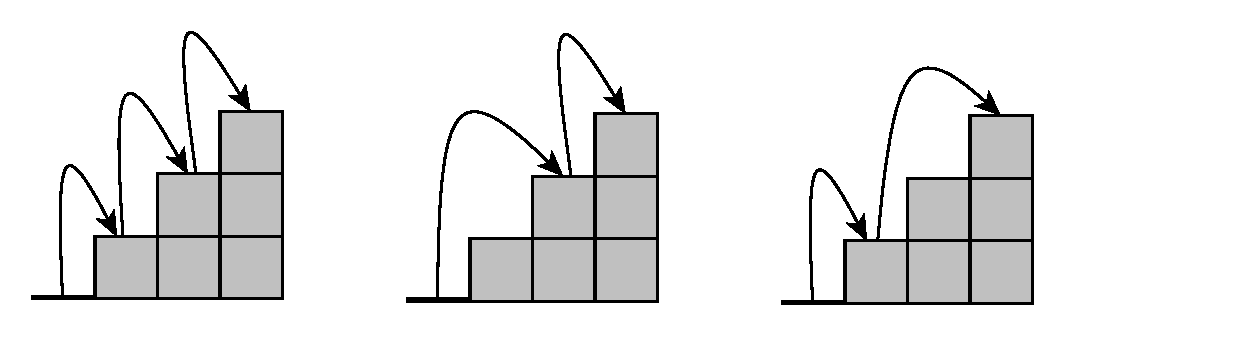
\includegraphics[width=\textwidth]{sources/stairs_climbing/images/stairs3}
	\caption{All different ways to climb a 3 stairs staircase using steps of size $1$ or $2$.}
	\label{fig:stair_example_3}
\end{figure}

\begin{figure}
	\centering
	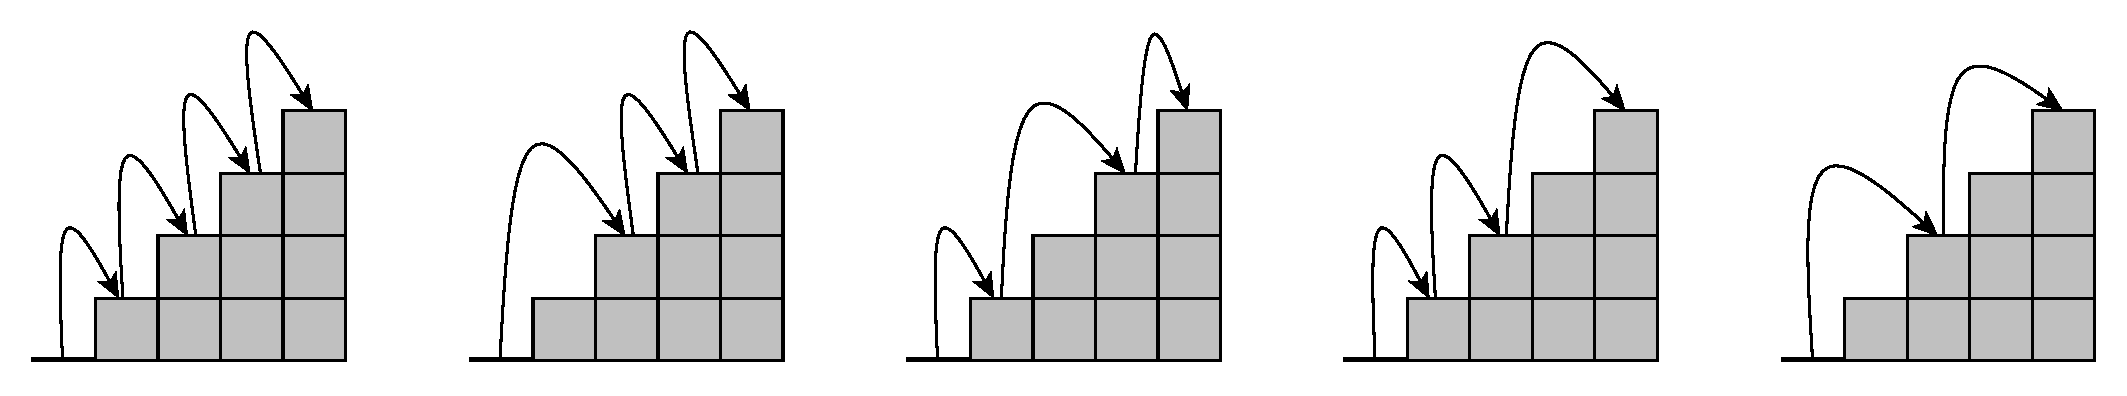
\includegraphics[width=\textwidth]{sources/stairs_climbing/images/stairs4}
	\caption{All different ways to climb a four stairs staircase using steps of size $1$ or $2$.}
	\label{fig:stair_example_5}
\end{figure}

\section{Clarification Questions}

\begin{QandA}
	\item \begin{questionitem} \begin{question} Can the size of the staircase be zero?  \end{question} 	 
    \begin{answered}
		\textit{Yes, the staircase can be made of zero steps.}
	\end{answered} \end{questionitem}
	
	\item \begin{questionitem} \begin{question} It is guaranteed that the answer will fit a built-in integer?  \end{question} 	 
    \begin{answered}
		\textit{Yes, do not worry about overflow.}
	\end{answered} \end{questionitem}

\end{QandA}

\section{Discussion}
\label{stairs_climbing:sec:discussion}

First, let's examine a few examples in order to identify the relevant patterns. Table \ref{tab:stairs_climbing_ways_up_tp_7} shows  how many ways there are to climb a stair of lenght $n$ up to $n=7$.

\begin{table}
	\centering
	\begin{tabular}{|c|c|}
		\hline
		$n$ & \textbf{Ways} \\ \hline
		$0$ & $0$ \\ \hline
		$1$ & $1$ \\ \hline
		$2$ & $2$ \\ \hline
		$3$ & $3$ \\ \hline
		$4$ & $5$ \\ \hline
		$5$ & $8$ \\ \hline
		$6$ & $13$ \\ \hline
		$7$ & $21$ \\ \hline
	\end{tabular}
\label{tab:stairs_climbing_ways_up_tp_7}
\caption{All the ways to climb a stair of length $n \leq 7$ }
\end{table}

Looking at the table one thing should be immediately apparent: the number of ways to climb the stair of size $n$ is equal to the $n^th$ element of the \textbf{Fibonacci} sequence (starting with two $1$).
Once that is clear then the solution is straightforward as shown in Listing \ref{list:stairs_climbing_fibonacci}.

\lstinputlisting[language=c++, caption=Solution to the stairs climbining problem with steps of size $1$ and $2$ using Fibonacci.,label=list:stairs_climbing_fibonacci]{sources/stairs_climbing/stairs_climbing_solution1.cpp}

Now, let's have a look at why the seemingly unrelated fibonacci sequence plays a role in this problem. If the problem is looked at as an iterative process in which at each step a certain number of stairs are climbed. For instance if $n = 3$ and:
\begin{itemize}
	\item[-] $1$ step is hopped then the number of remaining steps is $3-1 = 2$. 
	\item[-] $2$ steps are hopped then the number of remaining steps is $3-2 = 1$.
\end{itemize}
When one step is hopped, the problem changes from climbing $n$ stairs to $n-1$ stairs. At this point the problem is seemingly unchanged except for the number of stairs left to climb and the same reasoning can be applied again:
\begin{itemize}
	\item[-] $1$ step is hopped then the number of remaining steps is $(n-1)-1 = n-2$. 
	\item[-] $2$ steps are hopped then the number of remaining steps is $(n-1)-2 = (n-3)$.
\end{itemize}
As can be seen, two decisions are possible i.e. climbing one or two stairs, exactly as in the fibonacci sequence, until either the $n$ step or a point past it is reached.

\section{Common Variation
}
\subsection{Arbitrary step lengths}
\label{stairs_climbing:sec:arbitrary_steps}
What happens when the step sizes allowed are not just $1$ or $2$ but an array of $k$ positive values $A=\{s_1 < s_2 < \ldots < s_k\}$. The problem statement for this harder variant is as follows:

\begin{exercise}
You are climbing a stair case and it takes $n$ steps to reach the top.

Each time you can either climb $s_1$ or $s_2$ or $\ldots$ or $s_k$ steps where $0 < s_1 < s_2 < \ldots < s_k$. In how many distinct ways can you climb to the top?
\end{exercise}

The solution to this problem variant is equivalent to the easier version described in Section \ref{sec:stairs_climbing_statement_easy} when the allowed step sizes are $s_i = 1$ and $s_2=2$.

	
	%!TEX root = ../main.tex
%%%%%%%%%%%%%%%%%%%%%%%%%%%%%%%%%%
% Links: https://www.geeksforgeeks.org/sort-array-wave-form-2/
%
% Difficulty: Medium
% Companies: 
%%%%%%%%%%%%%%%%%%%%%%%%%%%%%%%%%%

\chapter{Wave Array}
\label{ch:wave_array}
\section*{Introduction}
The problem described in this chapter is often asked during one of the first stages of the onsite interview. It is not an hard problem and its implementation fits a few lines. and can therefore be completed very quickly if the right idea pops into the brain. 

\section{Problem statement}
\begin{exercise}
Given an array $A$ of $n$ integers, arrange the numbers in a wave-like fashion. 
In other words, sort the elements into a sequence such that $a_1 \geq a_2 \leq a_3 \geq a_4 \leq a_5 \geq \ldots$
\end{exercise}


\begin{example}
	\hfill \\
	Given $A= \{10, 5, 6, 3, 2, 20, 100, 80\}$ the followings are all valid output:
	\begin{itemize}
		\item[-]  \{20, 5, 10, 2, 80, 6, 100, 3\}
		\item[-]  \{10, 5, 6, 2, 20, 3, 100, 80\}
	\end{itemize}
\end{example}

\begin{example}
	\hfill \\
		Given $A= \{20, 10, 8, 6, 4, 2\}$ the followings are all valid output:
	\begin{itemize}
		\item[-] \{20, 8, 10, 4, 6, 2\}
		\item[-]  \{10, 8, 20, 2, 6, 4\}
	\end{itemize}
	
\end{example}

\begin{example}
	\hfill \\
	Given $A= \{10,9,8,7,6,5,4,3,2,1\}$ the following is a output: $\{10, 8, 9, 6, 7, 4, 5, 2, 3, 0, 1 \}$

\end{example}

\section{Clarification Questions}

\begin{QandA}
	\item Is the input only made of positive numbers?
	\begin{answered}
		\textit{No, the numbers can be positive or negative.}
	\end{answered}
	\item Are duplicates allowed?
	\begin{answered}
		\textit{Yes, duplicates might be present.}
	\end{answered}
	\item Do the numbers all lie in a particular range? If yes which one?
	\begin{answered}
		\textit{No assumptions can be made on the numbers.}
	\end{answered}
\end{QandA}

\section{Discussion}
\label{wave_array:sec:discussion}
The problem asks to return a copy of an array which elements are arranged in a particular form which reminds the one of a wave.
As usual with array problems, the first question should be asked is: how the problem become if the array is sorted?

\subsection{Sorting solution}
\label{wave_array:sec:sorting}

It turns out that in this case sorting the input makes the problem very easy. For all sorted array $A=\{a_1,a_2,\ldots\}$  the following holds: $A=\{a_0 \leq a-2 \leq \ldots \leq a_{n-1}\}$. If all elements with even index are swapped with the elements on their right the array as follows: $A=\{a_0 \geq a_2 \leq a_3 \geq a_4 \leq \ldots\}$ which is exactly how valid results are arranged. We can use this fact to solve this problem efficiently as shown in Listing \ref{list:wave_array_sorting}

\lstinputlisting[language=c++, caption=Solution to the wave array problem using sorting.,label=list:wave_array_sorting]{sources/wave_array/wave_array_solution1.cpp}

This is considered a good solution with time and space complexity of the code above is $O(nlog(n))$ and $O(n)$, respectively.
Note how only pairs of the form $(2i, 2i+1)$ are swapped (the variable $i$ is incremented by $2$ at the end of each iteration).

In some cases, the interviewer might, whenever there is more than one possible answer for a given input to return the lexicographically smallest. If it is the case the solution proposed below won't work and it should not be attempted.

\subsection{Linear time solution}
Despite the solution presented in Section \ref{wave_array:sec:sorting} is already good enough to impress the interviewer, there exists a solution that work in linear time and that is also easy to implementet as well as to explain. The core idea is that  elements at even index should always be greater than their adjacents neighbors. This can be enforced with a single pass on the array, by swapping elements at even indices if they happen to be smaller than their left and right neighbors. See Listing \ref{list:wave_array_linear} for a possible implementation of this idea.

\lstinputlisting[language=c++, caption=Linear time solutionto the wave array problem.,label=list:wave_array_linear]{sources/wave_array/wave_array_solution2.cpp}

This is considered a good solution\footnote{It will not work if the lexicographically smallest solution should be returned.} with optimal asymptotic complexity of $O(n)$ both in time and space.
Note how also in this case only pairs of the form $(2i, 2i+1)$ are swapped, and that each iteration takes case of arranging in a wave like fashion i.e. $A_{i-1} \geq A_i \leq A_{i+1}$.
	
    %%%%%%%%%%%%%%%%%%%%%%%%%%%%%%%%%%%%%%%%%%%%
	%               BIBLIOGRAPHY
	%%%%%%%%%%%%%%%%%%%%%%%%%%%%%%%%%%%%%%%%%%%%
	
	\chapter*{Bibliography}
	\addcontentsline{toc}{chapter}{\textcolor{ocre}{Bibliography}}
	\section*{Books}
	\addcontentsline{toc}{section}{Books}
	\printbibliography[heading=bibempty,type=book]
	\section*{Articles}
	\addcontentsline{toc}{section}{Articles}
	\printbibliography[heading=bibempty,type=article]
	
%%%%%%%%%%%%%%%%%%%%%%%%%%%%%%%%%%%%%%%%%%%%
%               INDEX
%%%%%%%%%%%%%%%%%%%%%%%%%%%%%%%%%%%%%%%%%%%%	
	\cleardoublepage
	\phantomsection
	\setlength{\columnsep}{0.75cm}
	\addcontentsline{toc}{chapter}{\textcolor{ocre}{Index}}
	\printindex


	%\backmatter

\end{document}